%%%%%%%%%%%%%%%%%%%%%%%%%%%%%%%%%%%%%%%%
% Classe do documento
%%%%%%%%%%%%%%%%%%%%%%%%%%%%%%%%%%%%%%%%

% Nós usamos a classe "unb-cic".  Deixe apenas uma das linhas
% abaixo não-comentada, dependendo se você for do bacharelado ou
% da licenciatura.

\documentclass[bacharelado]{unb-cic}
%\documentclass[licenciatura]{unb-cic}



%%%%%%%%%%%%%%%%%%%%%%%%%%%%%%%%%%%%%%%%
% Pacotes importados
%%%%%%%%%%%%%%%%%%%%%%%%%%%%%%%%%%%%%%%%

\usepackage[american, brazil]{babel}
\usepackage[T1]{fontenc}
\usepackage{indentfirst}
\usepackage{natbib}
\usepackage{xcolor,graphicx,url}
\usepackage[utf8]{inputenc}
\usepackage{amsmath,amssymb,amsthm}
\usepackage{verbatim}


%%%%%%%%%%%%%%%%%%%%%%%%%%%%%%%%%%%%%%%%
% Cores dos links
%%%%%%%%%%%%%%%%%%%%%%%%%%%%%%%%%%%%%%%%

% Veja o arquivos cores.tex se quiser ver que outras cores estão
% pré-definidas.  Utilizando o comando \hypersetup abaixo nós
% evitamos aquelas caixas vermelhas feias em volta dos links.

%%%%%%%%%%%%%%%%%%%%%%%%%%%%%%%%%%%%%%%%
% Cores do estilo Tango
%%%%%%%%%%%%%%%%%%%%%%%%%%%%%%%%%%%%%%%%

\definecolor{LightButter}{rgb}{0.98,0.91,0.31}
\definecolor{LightOrange}{rgb}{0.98,0.68,0.24}
\definecolor{LightChocolate}{rgb}{0.91,0.72,0.43}
\definecolor{LightChameleon}{rgb}{0.54,0.88,0.20}
\definecolor{LightSkyBlue}{rgb}{0.45,0.62,0.81}
\definecolor{LightPlum}{rgb}{0.68,0.50,0.66}
\definecolor{LightScarletRed}{rgb}{0.93,0.16,0.16}
\definecolor{Butter}{rgb}{0.93,0.86,0.25}
\definecolor{Orange}{rgb}{0.96,0.47,0.00}
\definecolor{Chocolate}{rgb}{0.75,0.49,0.07}
\definecolor{Chameleon}{rgb}{0.45,0.82,0.09}
\definecolor{SkyBlue}{rgb}{0.20,0.39,0.64}
\definecolor{Plum}{rgb}{0.46,0.31,0.48}
\definecolor{ScarletRed}{rgb}{0.80,0.00,0.00}
\definecolor{DarkButter}{rgb}{0.77,0.62,0.00}
\definecolor{DarkOrange}{rgb}{0.80,0.36,0.00}
\definecolor{DarkChocolate}{rgb}{0.56,0.35,0.01}
\definecolor{DarkChameleon}{rgb}{0.30,0.60,0.02}
\definecolor{DarkSkyBlue}{rgb}{0.12,0.29,0.53}
\definecolor{DarkPlum}{rgb}{0.36,0.21,0.40}
\definecolor{DarkScarletRed}{rgb}{0.64,0.00,0.00}
\definecolor{Aluminium1}{rgb}{0.93,0.93,0.92}
\definecolor{Aluminium2}{rgb}{0.82,0.84,0.81}
\definecolor{Aluminium3}{rgb}{0.73,0.74,0.71}
\definecolor{Aluminium4}{rgb}{0.53,0.54,0.52}
\definecolor{Aluminium5}{rgb}{0.33,0.34,0.32}
\definecolor{Aluminium6}{rgb}{0.18,0.20,0.21}

\hypersetup{
  colorlinks=true,
  linkcolor=DarkScarletRed,
  citecolor=DarkScarletRed,
  filecolor=DarkScarletRed,
  urlcolor= DarkScarletRed
}



%%%%%%%%%%%%%%%%%%%%%%%%%%%%%%%%%%%%%%%%
% Informações sobre a monografia
%%%%%%%%%%%%%%%%%%%%%%%%%%%%%%%%%%%%%%%%

\title{Uma proposta de Classificação de Recursos para a Arquitetura DSOA}

\orientador{\prof \dr Carla Denise Castanho}{CIC/UnB}
%\coorientador[a]{\prof[a] \dr[a] Coorientadora}{MAT/UnB}
\coordenador{\prof \dr Coordenador}{CIC/UnB}
\diamesano{23}{Julho}{2012}

\membrobanca{\prof \dr Professor I}{CIC/UnB}
\membrobanca{\prof \dr Professor II}{CIC/UnB}

\autor{Bruno Pessanha de}{Carvalho}
\coautor{Marcelo Valença de}{Almeida}
\CDU{004.4}

\palavraschave{ubíqua, classificação, dispositivos }
\keywords{ubiquitous, classification, devices}



%%%%%%%%%%%%%%%%%%%%%%%%%%%%%%%%%%%%%%%%
% Texto
%%%%%%%%%%%%%%%%%%%%%%%%%%%%%%%%%%%%%%%%

\begin{document}
  \maketitle
  \pretextual

  \begin{dedicatoria}
  Dedico a....
  \end{dedicatoria}

  \begin{agradecimentos}
  Agradeço a....
  \end{agradecimentos}

  \begin{resumo}
  A ciência...
  \end{resumo}

  \selectlanguage{american}
  \begin{abstract}
  The science...
  \end{abstract}
  \selectlanguage{brazil}

  \tableofcontents
  \listoffigures
  \listoftables

  \textual
  \chapter{Introdução}

\begin{figure}[ht]
	\center
	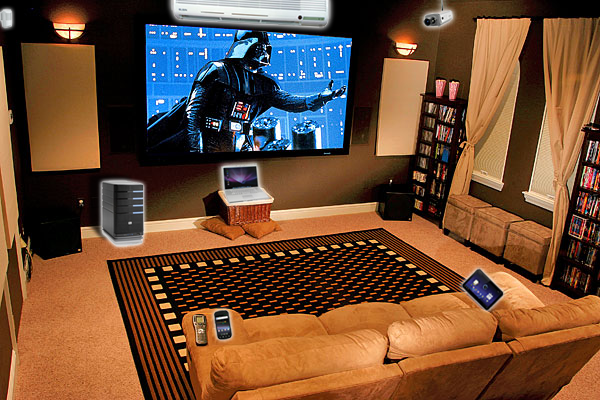
\includegraphics[scale=0.7]{imagens/salaUbiqua}
	\caption{Exemplo de ambiente inteligente.}
	\label{fig:ambienteInteligente}
\end{figure}

A computação ubíqua caracteriza-se por representar ambientes computacionais responsáveis por realizar determinadas tarefas predeterminadas de tal forma que certas premissas sejam obedecidas. Tais ambientes são normalmente compostos por um \emph{middleware} e diversas outras aplicações externas. Ao primeiro, cabe tratar e abstrair os detalhes das camadas inferiores e orquestrar as interações entre os diversos dispositivos espalhados pelo ambiente, enquanto que as aplicações devem tratar as interações realizadas junto aos usuários. É necessário que os componentes desse tipo de sistema trabalhem harmonicamente a fim de evitar, sempre que possível, toda e qualquer intervenção humana. A esta característica dá-se o nome de invisibilidade ~\cite{gomes2007, weiser1993, weiser1999}. Faz-se necessário, inclusive, que tais sistemas sejam pró-ativos ~\cite{gomes2007, buzeto2010} e consigam determinar, com a ajuda de informações de contexto previamente coletadas, quais as melhores decisões a serem tomadas em determinados instantes. Deve-se considerar, ainda, a mobilidade ~\cite{gomes2007, buzeto2010, weiser1999} dos aparelhos presentes e regidos dentro do ambiente em questão, a saber, o \emph{smart space}.

\begin{comment}
Em um ambiente inteligente se faz necessária a adaptabilidade de serviços de forma transparente para os clientes, ou seja, caso um serviço não esteja mais sendo provido por determinado dispositivo, o \emph{smart space} deve identificar esta falha e procurar um outro servidor ~\cite{gomes2007, passarinho2008, paranhos2009}.
\end{comment}

\begin{comment}
\section{DSOA}

Com o objetivo de auxiliar a modelagem de um \emph{smart space} levando em consideração as características de um ambiente ubíquo, foi criada a arquitetura DSOA(\emph{Device Service Oriented Architecture})~\cite{buzetoDSOA2010} que faz uso dos conceitos definidos na SOA(\emph{Service Oriented Architecture}) aplicados a um ambiente inteligente, onde recursos e serviços estarão disponíveis de forma dinâmica. Recursos, segundo a definição na proposta da DSOA, são um grupo de funcionalidades logicamente relacionadas que deverão ser acessíveis por meio de interfaces pré-definidas ~\cite{buzeto2010}. 

Esses recursos serão acessados por meio do \emph{middleware} \emph{uOS}, que utiliza um conjunto de protocolos \emph{uP} (\emph{Ubiquitous Protocols}) como interface de comunicação com \emph{drivers} de recursos disponíveis. A infra-estrutura implementada pelo \emph{uOS} para gerir os recursos do ambiente permite que uma aplicação de um dispositivo acesse recursos, apresentados na forma de um \emph{driver} (\emph{UosDriver}) de outros dispositivos presentes no ambiente.

Quando uma aplicação solicita um serviço de algum recurso, o \emph{uOS} deve tomar uma decisão sobre qual será o dispositivo detentor de tal recurso que provê o serviço solicitado que irá ser escolhido. Para que o \emph{uOS} possa tomar uma decisão inteligente sobre a escolha do dispositivo detentor do recurso, deseja-se que o tipo do recurso seja conhecido. Atualmente, a arquitetura DSOA/\emph{uOS} é pouco maleável nessa definição de tipo de recursos. Os recursos são definidos de forma linear, por exemplo: um recurso de \emph{mouse} com dois botões possui um \emph{driver} associado, já um \emph{mouse} com três botões, possui um outro \emph{driver} associado que não possui nenhuma relação com o primeiro, o que dificulta a tomada de decisão por parte do \emph{middleware}. Existem diversos padrões definidos que fazem uso de uma classificação de dispositivos ou recursos, mas não se adequam à arquitetura DSOA.

O objetivo deste trabalho é definir uma classificação de recursos e a partir desta classificação, prover uma hierarquia de recursos extensível para a arquitetura DSOA do \emph{middleware} de Computação Ubíqua \emph{uOS}. Essa hierarquia irá facilitar a escolha de determinado serviço provido por algum recurso por parte do \emph{uOS} ou de alguma aplicação cliente.
\end{comment}

Este trabalho está organizado da seguinte maneira: O capítulo 2 fundamenta os conceitos que serão utilizados neste trabalho. É iniciado apresentando uma visão geral do projeto UbiquitOS, explicando os principais conceitos da DSOA e mostrando em detalhes os protocolos que constituem o \emph{uP}. A seção seguinte mostra a importância da classificação de recursos bem como as diferentes maneiras de se classificar e representá-la. Ainda na segunda seção, serão apresentados alguns dos principais padrões conhecidos e projetos de Computação Ubíqua que utilizam uma classificação de recursos ou dispositivos para auxiliar em suas atividades. A seção e o capítulo são finalizados realizando um comparativo entre as diferentes classificações apresentadas. No capítulo 3 será apresentada a proposta de classificação deste trabalho e os impactos na arquitetura DSOA/\emph{uOS} e em seus protocolos.
  \chapter{Classificação de dispositivos}

Num ambiente em que dispositivos podem se movimentar livremente e cujos serviços devem ser compartilhados de forma transparente ao usuário, torna-se necessário que cada dispositivo presente na rede possa se comunicar facilmente com os demais, independente de quais tecnologias, padrões ou protocolos tenham sido adotados. É fundamental que essa comunicação seja feita de forma tão rápida e confiável quanto possível, pois toda atividade do \emph{middleware} com seus clientes depende dela, inclusive o processo de classificação dos recursos disponíveis no \emph{smart space}, ideia central deste documento.

\section{Formas de classificação}

Existem duas formas principais de realizar a classificação de dispositivos pretendida:

\begin{itemize}
	\item Fixa:
		Conjunto fixo de classificações não relacionadas.
	\item Relacionada:
		Estabelece relações entre os tipos básicos pré-definidos e suas especializações.

\end{itemize}

As classificações de forma Relacionada possuem a vantagem de reutilizar atributos definidos em outras classes e de poder adicionar novos atributos especializando os tipos relacionados, o que evita redundância na definição das classes. Enquanto as classificações de forma Fixa possuem a vantagem de serem mais simples de serem definidas.

Uma importante propriedade de uma classificação é a hierarquia, ou seja, uma representação em que as categorias da classificação podem ser especializadas formando novas categorias mais específicas, com diferentes atributos. Existem diferentes maneiras conhecidas de se representar uma hierarquia de forma a relacionar categorias que tenham atributos em comum: arquivos no formato XML, hierarquia de classes, ontologia ou simplesmente não utilizar uma hierarquia onde as categorias não tem relações entre si, caso da forma Fixa de classificação.

O XML (\emph{Extensible Markup Language}), como seu próprio nome sugere, pode ser estendido e dessa forma, é possível montar uma hierarquia de arquivos XML. O seu uso para descrever um tipo de dispositivo tem a vantagem de ser independente de plataformas de hardware ou software e, devido sua formatação, possui uma boa legibilidade, não necessitando de um pré-processamento por parte de um computador para seu conteúdo se tornar compreensível. Esse formato possui, contudo, a desvantagem de repetir uma grande quantidade de informação o que pode prejudicar a velocidade de comunicação entre dispositivos que o utilizem. Outro fator que deve ser levado em consideração é que o conjunto de protocolos \emph{uP} (\emph{Ubiquitous Protocols}) do \emph{middleware} \emph{uOS} utiliza o formato JSON para troca de mensagens, um mecanismo mais leve, e ainda assim estruturado, para representar informação.

A Hierarquia de Classes é amplamente utilizada em Programação Orientada à Objetos. Uma classe possui atributos ou propriedades e uma outra classe pode herdar esses atributos e criar uma especialização dessa classe raiz, à esse relacionamento dá-se o nome de Herança. Dependendo da linguagem orientada utilizada, uma Classe pode herdar métodos e atributos de várias outras Classes, formando uma herança múltipla de classes, ou então poderá cada Subclasse poderá herdar de apenas uma outra Classe, não podendo, entretanto, ocorrer uma herança circular, onde uma Classe A herda de uma Classe B, que por sua vez herda atributos de uma Classe C que especializa a Classe A. Uma Hierarquia de Classes forma, portanto, uma espécie de árvore de classes.

Ontologia é uma descrição formal de conceitos (classes) em um determinado domínio. Esses conceitos possuem propriedades, que descrevem atributos, características e restrições. De forma semelhante à orientação à objetos, conceitos podem possuir subclasses que especializam a classe superior. A Ontologia já permite uma herança múltipla de classes, e novos conceitos podem ser construídos por meio do relacionamento entre classes. Para construir uma Ontologia deve-se definir as classes do domínio, distribuir as classes de forma hierárquica, definir valores e restrições para suas propriedades e utilizar esses valores nas instâncias das classes da Ontologia. 

\begin{comment}
Dessa forma, temos uma base de conhecimento. As Ontologias se tornaram populares na Web por dividir produtos em categorias e em características em sites de venda, e atualmente são utilizadas para compartilhar informação entre pessoas e agentes inteligentes. Uma antologia provê reutilização de conhecimento e torna explícitas as hipóteses sobre um domínio e análise do domínio.
\end{comment}


\section{Padrões}
%Apresentar os padrões. Focar nas classificações feitas por eles, pontos fortes e fracos.

Nesta seção, discutir-se-á quatro dos principais protocolos e padrões pesquisados que fazem uso de uma classificação de recursos e utilizam as estratégias supracitadas para representar sua hierarquia de recursos: UPnP, IEEE 1451, DLNA e USB. 

\subsection{UPnP}
O \emph{Universal Plug and Play Protocol}(UPnP) é uma arquitetura para conectividade entre aplicações inteligentes, em execução em computadores e dispositivos \emph{wireless} em geral. Ela foi definida para facilitar a conectividade entre dispositivos em diferentes ambientes, como casas, pequenas empresas ou espaços públicos~\cite{upnpArch}. A arquitetura foi desenvolvida de forma a não necessitar de configurações e fornecer uma rede invisível com descoberta automática de dispositivos de diferentes fabricantes e diversas categorias. Dessa maneira, quando um novo dispositivo entra nessa rede, ele é identificado por um IP, publica seus serviços e conhece os serviços de outros dispositivos do ambiente. 

O UPnP utiliza o nome "Universal", pois não é necessária a utilização de ~\emph{drivers} para cada dispositivo. Para atingir esse objetivo, essa arquitetura faz uso de protocolos de internet bem conhecidos como IP, TCP, UDP, HTTP, além do formato XML, para facilitar a interoperabilidade entre dispositivos diversos. Da mesma forma que os protocolos de internet, os contratos dos serviços dos dispositivos são escritos em XML e enviados por HTTP.

Após a entrada do dispositivo em uma rede, ele recebe um IP via DHCP ou gera um IP para si, no caso de redes não gerenciadas. A \emph{UPnP Device Architecture}(UDA) divide os dispositivos em duas categorias principais: dispositivos controlados ou simplesmente "dispositivos" e pontos de controle~\cite{upnpArch} formando uma espécie de arquitetura cliente(pontos de controle)-servidor(dispositivos). 

\begin{comment}	
Quando um dispositivo entra na rede UPnP, ele comunica seus serviços para os pontos de controle ou, caso seja um ponto de controle, o protocolo de descoberta do UPnP permite que ele procure dispositivos de seu interesse. O segundo passo é o envio da descrição detalhada do dispositivo para os pontos de controle, que de posse dessa descrição podem enviar mensagens de controle para o dispositivo(passo 3). Os pontos de controle podem também assinar um contrato para envio de notificações de evento utilizando algum dos serviços que o dispositivo provê(passo 4). O último passo é de apresentação. Caso o dispositivo possua uma URL de apresentação é possível abrir uma página \emph{web} no \emph{browser} e um usuário pode controlar o dispositivo por meio dessa página~\cite{upnpArch}.
\end{comment}


Nosso foco neste trabalho se encontra no segundo passo do processo: a descrição dos dispositivos. Após sua descoberta, os pontos de controle ainda não têm muita informação sobre o dispositivo, então os pontos de controle interessados solicitam a descrição do dispositivo via uma URL que este dispositivo disponibilizou durante primeira etapa.

A descrição de um dispositivo definida no UPnP é feita por meio de um arquivo XML que inclui informações sobre o fabricante, lista de dispositivos embarcados ou serviços e para cada serviço, URLs para controle, eventos e apresentação. A descrição de serviços inclui ainda uma lista de comandos ou ações que o dispositivo deverá responder e para cada ação existem parâmetros ou argumentos. O estado do serviço é representado por uma lista de variáveis.

O UPnP define uma série de classificações pré-determinadas que os fabricantes podem utilizar na definição de seus dispositivos. Um característica encontrada nessas classificações é a sua leveza de serem implementadas por dispositivos com pouca capacidade de computação, embora também possam ser utilizadas por dispositivos mais robustos como computadores. São elas:

\begin{itemize}
\item Áudio/Vídeo:
	Essa categoria possui duas principais sub-classificações que foram sendo atualizadas com o desenvolvimento de novas tecnologias: 
	\begin{itemize}
		\item \emph{Media Server}:

			Define um dispositivo genérico que provê conteúdo de áudio e/ou vídeo, como CD e DVD \emph{players}, cameras, rádios, televisões e \emph{set-top boxes}. Embora, seja utilizado por dispositivos com diferentes capacidades de processamento e conteúdos, o \emph{Media Server} expõe conteúdo de forma consistente.

		\item \emph{Media Renderer}:

			Define um dispositivo genérico capazes de renderizar conteúdos de áudio e/ou vídeo como MP3 \emph{players} e televisões. Dependendo da implementação de um \emph{Media Renderer}, pode-se utilizar os recursos de auto-falante de uma televisão para consumir um serviço de música de um \emph{Media Server}.
	\end{itemize}
\item Gerenciamento de Dispositivos:
	Essa categoria foi criada para adicionar operações gerenciais à qualquer dispositivo UPnP. Esse gerência inclui funções para configuração de serviços e do próprio dispositivo, diagnóstico e correção de problemas além de gerência do \emph{firmware} e dos \emph{softwares} do dispositivo.

\item Automação Residencial:
	\begin{itemize}
		\item Cortina de Proteção Solar:

			Provê uma sombra por meio de uma cortina. Seu controle pode ser manual, automático ou desabilitado. Sua especificação não contempla configurações a respeito da automação da cortina ou proteções.
		\item Câmera Digital de Segurança:

			Provê controle básico sobre a configuração da câmera, contendo serviços de fotos e vídeos.
		\item Aquecimento, Ventilação e Ar Condicionado:
			
			Esse dispositivo conta com auxílio de sensores de temperatura e possui a capacidade de saber ou controlar a temperatura do ambiente por meio de ventiladores e ar-condicionados.
		\item Controles de Luz:
			
			São divididos em Luz binária, que representa uma lâmpada ou qualquer dispositivo emissor de luz que possa somente estar apagado ou aceso, e em Luz cuja intensidade pode ser alterada, 
	\end{itemize}

\item Rede:
	\begin{itemize}
		\item \emph{Gateway} de Internet:
			
			Essa classificação define um dispositivo de interconexão entre uma rede residencial local (LAN) e a \emph{Wide Area Network} (WAN), provendo conectividade com a internet.
			\begin{itemize}
				\item Dispositivo de Conexão WAN: É um dispositivo virtual definido tendo o \emph{Gateway} de Internet como raiz. Funciona como um contêiner para um \emph{link} ou serviços de conexão em uma interface WAN. 
				\item Dispositivo WAN: É um dispositivo virtual efinido tendo o \emph{gateway} de internet como raiz. Cada dispositivo WAN é uma instância virtual de uma interface WAN no \emph{gateway} de internet. Múltiplas interfaces físicas WAN para clientes UPnP, existirão distintas instâncias deste dispositivo.
			\end{itemize}

		\item Ponto de acesso WLAN(\emph{Wireless Local Area Netowork}):
			
			Esse dispositivo implementa os padrões IEEE 802.11 (a,b,g) sem fio para prover uma infraestrutura de rede para casas e pequenas empresas. Essa definição não inclui uso dos pontos de acesso como \emph{hotspots} ou redes de grandes empreendimentos. O ponto de acesso age com uma ponte \emph{Ethernet} que permite ligações de múltiplos nós com a LAN.
	\end{itemize}

\item Impressora:
	Define um dispositivo com capacidade de impressão. Essa especificação não abrange dispositivos que possuem funções de FAX ou \emph{Scanner}, que possui uma especificação própria.

\item Acesso Remoto:
	Essa categoria é dividida entre dois dispositivos:
	\begin{itemize}
		\item Agente de Descoberta de Acesso Remoto:

			Possui a função de prover a capacidade de sincronizar a informação sobre a descoberta UPnP entre duas redes remotas.
		
		\item Servidor de Acesso Remoto:
		
			Permite que pontos de controle configurem Servidores de Acesso Remoto.

	\end{itemize}

\item Interface Remota:
	Classifica dispositivos entre servidores e clientes de uma interface remota com o usuário.

\item \emph{Scanner}:
	Representa um dispositivo de \emph{Scanner} com \emph{feeder} opcional. Esse dispositivo possui os serviços de digitalização via \emph{feeder} ou \emph{flatbed} e um serviço para configuração com o painel frontal do dispositivo. Essa categoria não contempla funcionalidades de Fax ou cópias.

\item Telefonia:
	\begin{itemize}
		\item Servidor de Telefonia:

			Permite que pontos de controle gerenciem chamadas telefônicas, mensagens e presença por meio de outros dispositivos UPnP. 

		\item Cliente de Telefonia:
		
			Permite que pontos de controle possam gerenciar mídias por meio de um de um servidor de telefonia.
				
	\end{itemize}

\item Básico:
	A definição de dispositivos básicos provêm um mecanismo para produtos que não se enquadram em uma classificação adequada do UPnP, possam utilizá-lo. Por esse motivo, essa especificação não possui nenhum serviço definido, mas pode ser utilizada como dispositivo raiz para outras categorias já definidas.
\end{itemize}

Os fabricantes podem, a partir de uma classificação padrão, estender e especializar determinada definição adicionando novos serviços, por exemplo, o que sugere uma hierarquia de dispositivos por meio de arquivos XML. Um fator interessante nas classificações de dispositivos UPnP é que sua especificação já traz consigo a especificação de serviços que esses dispositivos provêm. 

\subsection{IEEE 1451}
O IEEE 1451 se divide em uma família de padrões que foram criados com os objetivos de permitir a capacidade de comunicação entre transdutores(sensores e atuadores) de forma \emph{plug-and-play} por meio de redes com ou sem fio, facilitar a criação de transdutores com inteligência embarcada, simplificar a configuração e manutenção de sistemas, prover comunicação entre transdutores legados, e por fim, habilitar a implementação de transdutores inteligentes e com uso mínimo de memória~\cite{ieee1451journal}.

Um dos padrões da família, o IEEE 1451.1, define um modelo de informação para \emph{Network Capable Application Processors} (NCAP) que foi estabelecido para especificar um modelo de objetos comum e interfaces de componentes da rede de transdutores. Dessa forma, foi desenvolvido um \emph{framework} orientado a objetos que pode ser estendido para facilitar o desenvolvimento de aplicações que foi definido da seguinte forma: Um modelo de dados que especifica a forma e o tipo de comunicação, tanto local quanto remota, por meio das interfaces de objetos 1451.1, um modelo de objetos que especifica tipos de componentes de software usados para definir e implementar sistemas e, por fim, modelos de comunicação que definem a sintaxe e semântica das interfaces de software entre redes de comunicação e objetos de aplicação~\cite{ieeeOO1451}~\cite{ieee1451monitoring}.

\begin{figure}[ht]
\center
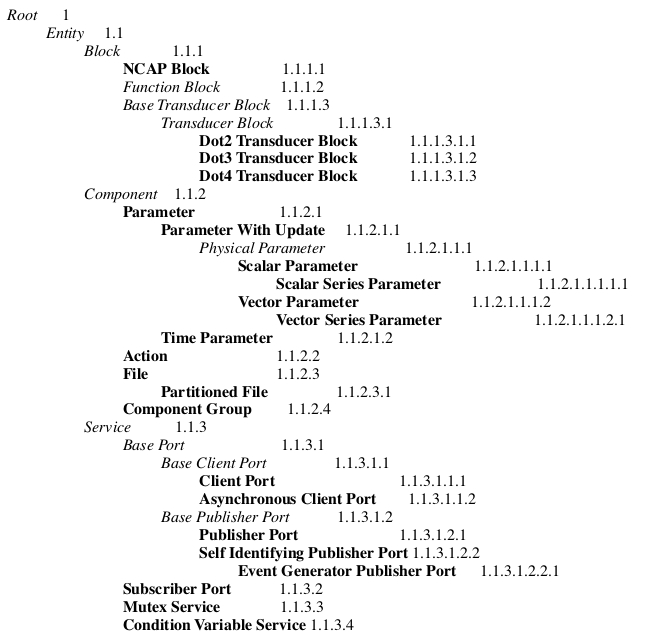
\includegraphics[scale=0.5]{imagens/ieee1451-classHierarchy}
\caption{Hierarquia de Classes do Padrão IEEE 1451.1}
\label{fig:classHierarchy}
\end{figure}

O padrão ~\cite{ieee1451standard} especifica cada classe no modelo definindo as interfaces da classe(por meio de assinaturas e operações) e o comportamento da classe (via texto ou máquinas de estado). A figura~\ref{fig:classHierarchy} mostra a hierarquia de classes definida pelo padrão em que as classes em itálico representam classes abstratas. Nesta figura é possível observar 3 tipos principais de objetos IEEE 1451.1:

\begin{itemize}
	\item\emph{Block}:

	Especializada em três classes:
		\begin{itemize}
			\item\emph{NCAPBlock}:
				Provê interfaces para comunicações de rede e configurações do sistema.
			\item\emph{BaseTransducerBlock}:
				Provê interfaces entre transdutores e funções.
			\item\emph{FunctionBlock}:
				Provê encapsulamento de funções específicas.
		\end{itemize}
	
	\item\emph{Component}:
	
		Fornecem:
		\begin{itemize}
			\item Informações estruturadas: medidas e arquivos.
			\item Coleções de objetos relacionados com a aplicação.
			\item Ações com estados onde a ação é executada após um período de tempo.
		\end{itemize}
	\item\emph{Service}:
	
		Suportam:
		\begin{itemize}
			\item Comunicação entre objetos de diferentes NCAPs.
			\item Sincronização do sistema.
		\end{itemize}
\end{itemize}

Há ainda as classes não-IEEE 1451.1, que não estão representadas na Figura ~\ref{fig:classHierarchy} e possuem restrições de aplicabilidade na arquitetura IEEE 1451.



\subsection{DLNA}

A \emph{Digital Living Network Alliance} (DLNA) é uma organização composta pelas principais empresas de eletrônicos de consumo, computação e dispositivos móveis. Foi fundada em 2003 e tem como objetivo fornecer orientações para permitir a interoperabilidade entre dispositivos para completar a convergência da indústria digital, levando, dessa forma, inovação, simplicidade e valor para os consumidores~\cite{dlnaoverview}. Tem como visão facilitar a criação, o gerenciamento e o compartilhamento de conteúdo digital (fotos, músicas e vídeos) entre os dispositivos pertencentes à mesma rede~\cite{dlnahdvideostreaming}. Deve permitir, por exemplo~\cite{dlnaoverview}:

\begin{itemize}
	\item Facilmente adquirir, armazenar e acessar música digital a partir de praticamente qualquer lugar da casa;
	\item Facilmente gerenciar, visualizar, imprimir e compartilhar fotos digitais;
	\item Transportar seu conteúdo favorito a partir qualquer lugar, mesmo que as pontas envolvidas estejam em movimento;
	\item Aproveitar a gravação e reprodução de conteúdo distribuído e multi-usuário.
\end{itemize}

Imagine, por exemplo, uma situação hipotética em que uma pessoa deseja compartilhar um pequeno vídeo com seus amigos a partir de seu celular. A fim de exibir esse vídeo em sua TV widescreen na sua sala de estar, ela necessita, primeiramente, envia-lo para seu próprio email. Em seguida, deve ligar seu PC, fazer o download do vídeo e salvá-lo em um \emph{pendrive} ou cartão de memória. Posteriormente, deve ligá-lo na TV ou em um receptor digital e, então, utilizar a interface do dispositivo para localizar o vídeo e exibi-lo~\cite{dlnahdvideostreaming}.

\begin{figure}[ht]
	\center
	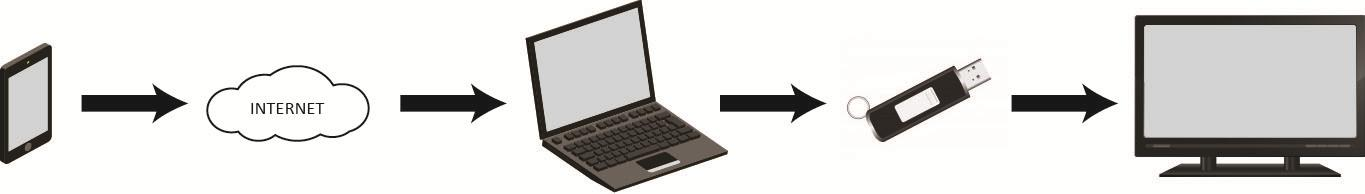
\includegraphics[scale=0.3]{imagens/dlna1}
	\caption{A exibição de um vídeo ou foto de um celular em uma TV envolve tal processo tradicional, tedioso e demorado que os consumidores raramente farão.}
	\label{fig:traditionalProccess}
\end{figure}

Além de interromper a conversa, esse tipo de processo de tranferência de conteúdo simplesmente consome muito tempo, mesmo quando ocorre sem problemas. Como resultado, a partilha informal de vídeo em múltiplas telas não é visto muitas vezes como uma opção razoável~\cite{dlnahdvideostreaming}.

Este é o valor da proposição que o DLNA oferece aos seus consumidores: a partilha contínua e sem esforço de conteúdo digital. Produtos projetados seguindo as diretrizes DLNA estabelecidas para compartilhar vídeo em apenas um único passo: a transmissão de uma cópia do vídeo do telefone sem fio para a TV. O consumidor pode até mesmo congelar o vídeo usando um "controle remoto" do menu no telefone, bem como \emph{fast-forward} e reproduzir o vídeo~\cite{dlnahdvideostreaming}.

\begin{figure}[ht]
	\center
	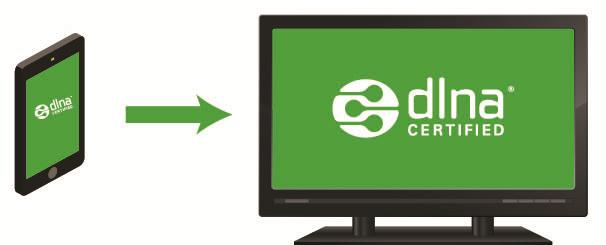
\includegraphics[scale=0.3]{imagens/dlna2}
	\caption{O valor da proposição do DLNA é o compartilhamento transparente e fácil de conteúdo, permitindo que os consumidores enviem uma cópia de um vídeo ou fotos diretamente para a TV em uma única etapa.}
	\label{fig:dlnaProccess}
\end{figure}

Suas diretrizes destacam casos de uso cuidadosamente construídos para redes domésticas (veja a tabela~\ref{tab:casosdeuso_dlna}), funções adicionais que aumentam a experiência do compartilhamento de conteúdo e doze classes de dispositivos espalhados na categoria "Rede Doméstica e Dispositivos Móveis". A classificação de um dispositivo é feita de tal forma que um único aparelho multifuncional pode possuir diversas categorias diferentes~\cite{dlnahdvideostreaming}.

Em suma, o DLNA pode ser visto como uma coleção de padrões abertos que definem como uma rede residencial interage em todos os seus níveis, ou seja, além de definir como os diferentes padrões irão interoperar e como os dados serão tratados em cada nível, ele também reduz o número de padrões que um dispositivo deve suportar.

\begin{table}
	\begin{center}
		\begin{tabular}{rl}
		\hline
		\textbf{Casos de Uso} & \textbf{Exemplo}																\\
		\hline
		Enviar & Tranferir vídeos ou imagens capturadas em uma câmera digital ou celular para um computador.	\\
		\hline
		Empurrar & Exibir vídeos ou imagens capturadas em uma câmera digital ou celular diretamente em uma TV sem intermédio de um computador. \\
		\hline
		Localizar e Reproduzir ou "Reproduzir em..."" & Utiliza um celular para localizar uma música ou vídeo armazenados em um computador, unidade de disco externa ou um dispositivo \emph{Network-Attached Storage} (NAS) e transferi-lo, via \emph{stream} ou não, para reprodução. \\
		\hline
		Puxar e imprimir ou "Imprimir em..." & Vizualizar na TV uma foto armazenada em um servidor de mídia e imprimi-la utilizando uma impressora em rede. \\
		\hline
		\end{tabular}
	\end{center}
	\caption{Exemplos de casos de uso~\cite{dlnahdvideostreaming}.}
	\label{tab:casosdeuso_dlna}
\end{table}

\begin{table}
	\begin{center}
		\begin{tabular}{rll}
		\hline
		\textbf{Camada} & \textbf{Função definida} & \textbf{Padrões}				\\
		\hline
		Transmissão Protegida & Como um conteúdo comercial está protegido em uma rede doméstica. & DTCP/IP \\
		\hline
		Formatos de Mídia & Como um conteúdo de mídia está codificado e identificado para interoperabilidade. & MPEG2, MPEG4, AVC/H.264, LPCM, MP3, AAC LC, JPEG, XHTML-Print- \\
		\hline
		Transporte de Mídia & Como um conteúdo de mídia é transferido. & HTTP, Quality of Service \\
		\hline
		Gerência de Mídia & Como um conteúdo de mídia é identificado, gerenciado e distribuído. & UPnP AV 1.0, UPnP Print Enhanced 1.0 \\
		\hline
		Descoberta e Controle & Como dispositivos se descobrem e se controlam um ao outro. & UPnP Device Architecture 1.0 \\
		\hline
		Redes IP & \multirow{2}{*}{Como dispositivos com e sem fio fisicamente se conectam e se comunicam.} & IPv4 Protocol Suite \\
		Conectividade & & Wired: Ethernet 802.3, MoCAWireless: Wi-Fi 802.11, Wi-Fi Protected Setup \\
		\hline
		\end{tabular}
	\end{center}
	\caption{Camadas padrões DLNA~\cite{dlnahdvideostreaming}.}
	\label{tab:camadaspadroes_dlna}
\end{table}
\subsection{USB}

O \emph{Universal Serial Bus} (USB) é uma arquitetura de comunicaçao que adiciona a uma máquina hospedeira a capacidade de se interconectar a uma variedade de dispositivos. Surgiu com o intuito de sanar três das principais dificuldades enfrentadas à época de sua criação~\cite{usbspec}:

\begin{itemize}
	\item Integrar as plataformas das industrias da informática e comunicação. Para tal, a troca de informações entre esses dispositivos deveria acontecer de forma ubíqua e barata;
	\item Facilitar a reconfiguração de dispositivos de um computador, tais como teclados, mouses e joysticks;
	\item Integrar todas as interfaces existentes à época em um única que pudesse ser utilizada pela maior quantidade possível de dispositivos: telefone, fax, modem, adaptadores, secretárias eletrônicas, \emph{scanners}, PDA's, teclados, \emph{mouses}, etc.
\end{itemize}

De acordo com sua especificação, suas máquinas hospedeiras devem:

\begin{itemize}
	\item Fornecer energia aos seus periféricos;
	\item Suportar todas as velocidades definidas (SuperSpeed, Low Speed, Full Speed e High SuperSpeed);
	\item Suportar todos os tipos de fluxo de dados definidos (controle, massa, interrupção e síncrono).
\end{itemize}

Entende-se por máquina hospedeira qualquer dispositivo possuidor dos recursos necessários para realizar esta função. Por exemplo, conectar uma câmera à uma impressora faz sentido, enquanto que conectar um GPS à mesma impressora, não. Assim sendo, cada máquina hospedeira não necessita se comportar exatamente como um computador, mas apenas servir como hospedeiro a certos dispositivos convenientes~\cite{usb3spec}.

Atualmente sua velocidade de comunicação varia entre 1.5 ou 12 megabits por segundo (mbs) e seu protocolo permite configurar dispositivos durante a fase de inicialização ou quando eles são plugados em tempo de execução~\cite{hid}, deixando toda parte pesada desse processo a cargo do hospedeiro~\cite{usb3spec}. Tais dispositivos são divididos em várias classes e/ou subclasses diferentes (veja a tabela~\ref{tab:dispositivos_usb}), cada qual definindo um comportamento e protocolos comuns para dispositivos que oferecem funções similares~\cite{hid}.

Um mesmo dispositivo USB pode pertencer a uma ou múltiplas classes. Por exemplo, um celular pode utilizar atributos da classe HID, Audio e Comunicação. A partir dessas divisões será possível estabelecer uma hierarquia, a qual poderá ser usada no processo de classificação dos dispositivos presentes no smartspace.

Seguem abaixo as classes existentes juntamente com suas descrições~\cite{usbclasscodes}.

\begin{comment}
\begin{table}
	\begin{center}
		\begin{tabular}{cccc}
		\hline
		\multicolumn{4}{c}{\textbf{Classes de Dispositivos}}													\\
		\hline
		Audio					&	Comunicação				&	Interface Humana (HID)	&	Físico 				\\
		\hline
		Imagem					&	Impressora				&	Disco Rígido			&	Hub 				\\
		\hline
		\emph{Smart Card}		&	Segurança de Conteúdo	&	Vídeo					&	Saúde Pessoal 		\\
		\hline
		Diagnóstico				&	Controlador Wireless	&	Diversos				&	Aplicação Específica\\
		\hline
		Fabricante Específico	&							&							&						\\
		\hline
		\end{tabular}
	\end{center}
	\caption{Exemplos de classes de dispositivos USB~\cite{usbclasscodes}.}
	\label{tab:dispositivos_usb}
\end{table}
\end{comment}

\begin{itemize}
	\item \emph{Audio}: destina-se a todos os dispositivos ou funções embutidos em aparelhos que são usados para manipular áudio, voz e quaisquer funcionalidades relacionadas. Isso inclui tanto dados de áudio (analógico e digital) quanto a capacidade de diretamente controlar tal ambiente por meio de controles de volume e tom. Não inclui a funcionalidade para operar mecanismos de transporte que estão relacionados com a reprodução de dados de áudio, tais como mecanismos de transporte de fita ou controles de unidade de CD-ROM~\cite{usbaudioclass}.

	Exemplos de tais dispositivos incluem \emph{headsets}, \emph{headphones} and \emph{microphones}~\cite{usbbasicaudioclass}.
	\item \emph{Communications and CDC Control}: há três classes que compõem a definição de dispositivos de comunicação: a Classe de Comunicação do Dispositivo, a Classe de Interface de Comunicação e a Classe de Interface de Dados. A primeira é uma definição de nível do dispositivo e é utilizada pelo hospedeiro para identificar corretamente um dispositivo de comunicação que pode apresentar diferentes tipos de interfaces. A segunda define um mecanismo de propósito geral que pode ser utilizado para habilitar todos os tipos de serviços de comunicação sobre o Universal Serial Bus (USB). A última define um mecanismo de propósito geral para permitir a transferência em massa quando os dados não atendem aos requisitos para qualquer outra classe~\cite{usbcommunicationclass}.

	Exemplos de tais dispositivos incluem:
	\begin{itemize}
		\item Telecomunicações: modens analógicos, adaptadores de terminais ISDN, telefones digitais e telefones analógicos;
		\item Dispositivos de rede: modens ADSL, modens à cabo, adaptadores/hubs \emph{Ethernet} 10BASE-T e \emph{Ethernet} cross-over cabos.
	\end{itemize}
	\item HID (\emph{Human Interface Device}): destina-se primordialmente aos dispositivos que são usados por humanos para controlar e operacionalizar quaisquer tipos de sistemas computacionais~\cite{hid}. Mais específicamente, possui as seguintes particularidades:
	\begin{itemize}
		\item Deve ser tão compacto quanto possível para evitar desperdício de espaço no dispositivo;
		\item Permitir a aplicação de software para evitar informação desconhecida;
		\item Ser extensível e robusto;
		\item Suportar hierarquias e coleções;
		\item Ser autodescritivo para permitir aplicações de software genéricos.
	\end{itemize}

	Exemplos de tais dispositivos incluem: teclados e dispositivos apontadores, painéis de controle, controles que podem ser encontrados em dispositivos como telefones, controles remotos, jogos ou dispositivos de simulação e aparelhos que não necessitam de interação humana mas que fornecem dados de forma similar aos dipositivos da classe HID~\cite{hid}.
	\item \emph{Physical}: é vista como uma extensão da classe HID para dispostivos que requerem resposta física em "tempo real". Seu foco principal está em dispositivos táteis e na implementação de sistemas com resposta à força. Contúdo, não há exigência de que os membros desta classe gerem esse tipo de efeito~\cite{usbphysicalclass}.

	Exemplos de tais dispositivos incluem: \emph{joysticks} e plataformas de movimento.
	\item \emph{Image}: 
	\item \emph{Printer}: 
	\item \emph{Mass Storage}: 
	\item \emph{Hub}: 
	\item \emph{CDC-Data}: 
	\item \emph{Smart Card}: 
	\item \emph{Content Security}: 
	\item \emph{Video}: 
	\item \emph{Personal Healthcare}: 
	\item \emph{Diagnostic Device}: 
	\item \emph{Wireless Controller}: 
	\item \emph{Miscellaneous}: 
	\item \emph{Application Specific}: 
	\item \emph{Vendor Specific}: 
\end{itemize}

\begin{comment}
Com o sucesso do protocolo, novas categorias surgiram gradualmente como alternativas às novas tecnologias e/ou aos novos dispositivos. Seguem:

\subsubsection{\emph{SuperSpeed}}

Como efeito do avanço tecnológico, o desenvolvimento dos novos tipos de dispositivos, dos formatos de mídia e dos armazenamentos de baixo custo está convergindo. Para tal, requer largura de banda significativamente maior para manter uma experiência do usuário aceitável. E o USB 3.0 atende essa necessidade adicionando uma taxa de transferência ainda maior para suprir essa demanda. Traz melhorias significativas de desempenho ao consagrado USB padrão, mantendo-se compatível com os diversos outros dispositivos USB espalhados pelo mercado. Além de melhorar a eficiência de energia, sua taxa de transferência será até dez vezes maior que a taxa de transferência do USB \emph{Hi-Speed}~\cite{usbsuperspeed}.

\subsubsection{Wireless}



\subsubsection{Hi-Speed}



\subsubsection{On-The-Go and Embedded Host}

Dentre as diversas classes existentes, uma em especial chama a atenção: \emph{Human Interface Device} (HID). Esse tipo de classe, de forma geral, destina-se primordialmente aos dispositivos que são usados por humanos para controlar e operacionalizar quaisquer tipos de sistemas computacionais~\cite{hid}. Mais específicamente, possui as seguintes particularidades:

\begin{itemize}
	\item Deve ser tão compacto quanto possível para evitar desperdício de espaço no dispositivo;
	\item Permitir a aplicação de software para evitar informação desconhecida;
	\item Ser extensível e robusto;
	\item Suportar hierarquias e coleções;
	\item Ser autodescritivo para permitir aplicações de software genéricos.
\end{itemize}

\begin{table}
	\begin{center}
		\begin{tabular}{lr}
		\hline
		\textbf{Dispositivo} & \textbf{Exemplo Descritivo} \\
		\hline
		Teclados e dispositivos apontadores & Mouses, trackballs e joysticks \\
		Painéis de controle & Maçanetas, Interruptores, botões e alavancas \\
		Controles que podem ser encontrados \\
		em dispositivos como telefones,\\
		controles remotos, jogos ou dispositivos \\
		de simulação & Luvas virtuais, câmbios, \\
		volantes e pedais \\
		Dispositivos que não necessitam de \\
		interação humana mas que fornecem dados \\
		de forma similar aos dipositivos da \\
		classe HID & Leitores de códigos de barra, \\termômetros ou voltímetros. \\
		\hline
		\end{tabular}
	\end{center}
	\caption{Exemplos de classes de dispositivos USB.}
	\label{tab:dispositivos_USB}
\end{table}
\end{comment}

\section{Estado da Arte}
Nesta seção, apresentaremos alguns projetos de computação ubíqua e mostraremos como esses projetos tratam a classificação de recursos.

\subsection{Gaia}
No projeto Gaia foi criado um middleware com o objetivo de dar suporte ao desenvolvimento e execução de aplicações portáveis em \emph{Active Spaces}, ambientes com sistemas interativos, o Gaia OS, uma abstração de um sistema operacional. O middleware foi projetado para ser uma infraestrutura distribuiída que coordena entidades de software e dispositivos heterogêneos em um \emph{smart space}. O Gaia OS expõe serviços para buscar e utilizar recursos presentes no ambiente, ter conhecimento do contexto e provê um \emph{framework} para desenvolver aplicações móveis sensíveis ao contexto, que conheçam os recursos disposníveis, utilizem múltiplos dispositivos e tenham como foco o usuário~\cite{gaia2002}.

\emph{Active Spaces} são espaços físicos como escritórios, salas de conferência, casas, hospitais, campi, cidades que possuem dispositivos integrados ao ambiente. O objetivo desses dispositivos é prover e obter informação sobre usuários do ambiente, os ajudando a realizar tarefas que eles não poderiam sem os dispositivos, ou facilitando tarefas do cotidiano.

\begin{figure}[ht]
\center
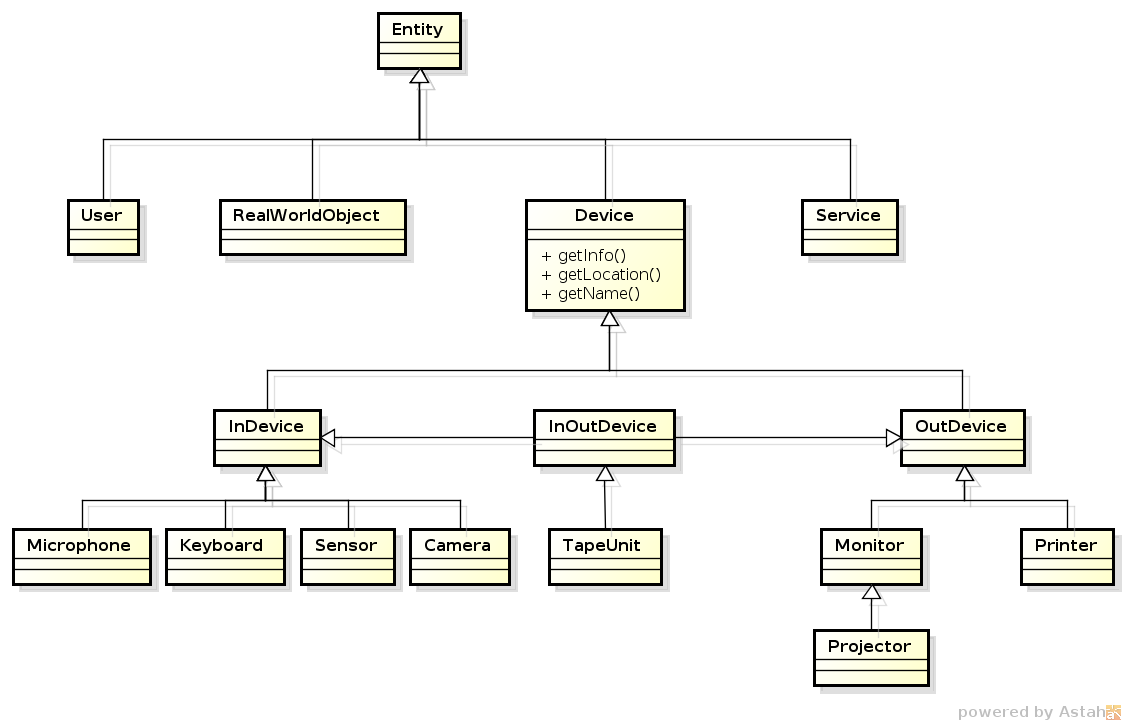
\includegraphics[scale=0.5]{imagens/gaia-devices}
\caption{Diagrama de Classes Simplificado~\cite{gaiaDevices}}
\label{fig:gaiaClassDiagram}
\end{figure}

No projeto, foi desenvolvido um \emph{framework} para a interação entre dispositivos heterogêneos. Esse \emph{framework} permite a representação das interfaces dos dispositivos com diferentes níveis de detalhe e especialização. As interfaces são definidas utlizando IDL(\emph{Interface Description Language}), que permite a construção de \emph{drivers} de dispositivos em qualquer linguagem de programação. 

A figura~\ref{fig:gaiaClassDiagram} mostra o Diagrama de Classes simplificado do projeto Gaia. Podemos observar que a Classe \emph{Device} é especializada em dispositivos de entrada(\emph{InDevice}) e saída(\emph{OutDevice}) de dados. Os dispositivos de entrada são ainda especializados em: Microfone, Câmera, Teclado e Sensor, enquanto os dispositivos de saída são especializados em: Impressora e Monitor, que por sua vez, é especializado em Projetor. Há ainda a interface para dispositivos que são de entrada e saída que é especializada em uma unidade de Fita.

\begin{comment}
http://gaia.cs.uiuc.edu/html/device.htm
http://gaia.cs.uiuc.edu/papers/GaiaSubmitted3.pdf
\end{comment}

\subsection{Amigo}
O projeto Amigo (\emph{Ambient Intelligence for the Networked home environment}) desenvolveu um \emph{middleware} com arquitetura baseada em SOA que integra dinamicamente sistemas heterogêneos para alcançar a interoperabilidade entre serviços e dispositivos. O middleware provê a semântica para comunicação e descoberta de dispositivos e serviços disponíveis no ambiente, incluindo dispositivos que utlizam padrões para descoberta como o UPnP integrando dispositivos móveis, computadores pessoais, eletrodomésticos e dispositivos de automação residencial~\cite{amigoArch}.

\begin{figure}[ht]
\center
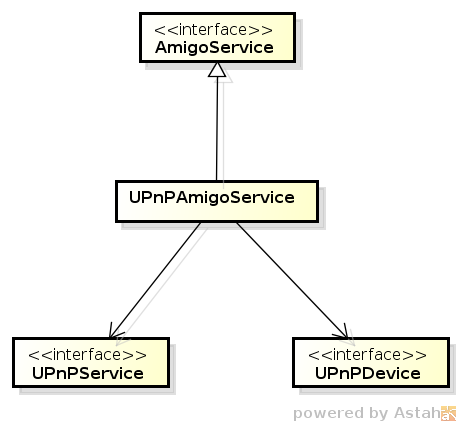
\includegraphics[scale=0.5]{imagens/amigo-interfaces}
\caption{Implementação de um \emph{AmigoService} utilizando serviços UPnP~\cite{amigoCore}}
\label{fig:amigoInterfaces}
\end{figure}

Além de utilizar o UPnP para a descoberta de dispositivos, o Amigo é compatível com as classificações de dispositivos do UPnP. Quando um dispositivo UPnP é encontrado, é criada uma instância de um \emph{UPnPDevice} e o \emph{driver AmigoUPnP} é notificado e executa o método \emph{getServices} do \emph{UPnPDevice} e cria para cada serviço uma instância do \emph{UPnPAmigoService}. A figura~\ref{fig:amigoInterfaces} mostra o relacionamento entre as interfaces UPnP com a implementação de uma interface de um Serviço do Amigo.

Os serviços do Amigo são modelados em uma Ontologia que é utilizada para comparar serviços e decidir se eles são equivalentes. A classe central da Ontologia é o Componente que representa o dispositivo provê o serviço. Para representar o que o dispositivo requer e provê, foi introduzido o conceito da Capacidade, dividida em Capacidade Requuerida e Capacidade Provida. Uma Capacidade possui parâmetros de entrada e saída que também são modelados em classes. As capacidades são então associdas à Conversas suportadas pelo Componente e relacionadas à mensagens que são empregadas na Conversa associada como mostra a figura ~\ref{fig:amigoServiceOntology}.

\begin{figure}[ht]
\center
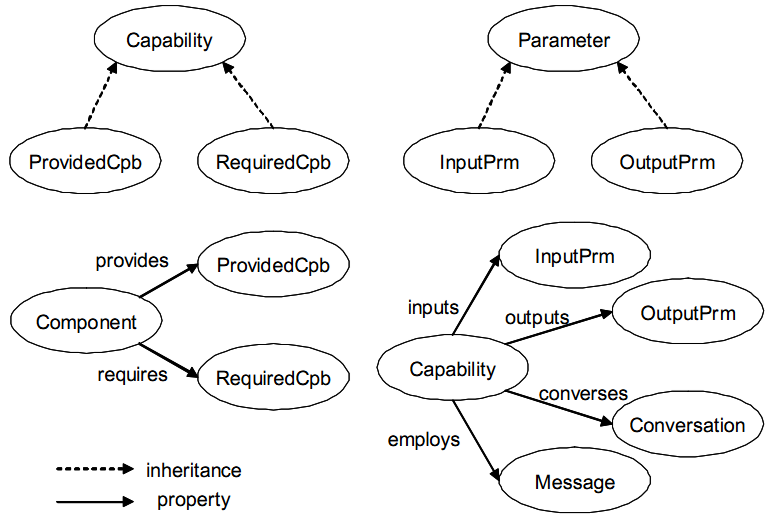
\includegraphics[scale=0.5]{imagens/amigo-ontology}
\caption{Elementos básicos da Ontologia de Serviços~\cite{amigoCore}}
\label{fig:amigoServiceOntology}
\end{figure}


\begin{comment}
http://www.hitech-projects.com/euprojects/amigo/publications/IST-004182%20Amigo-IP%20short%20project%20description.pdf
http://www.hitech-projects.com/euprojects/amigo/deliverables/Deliverable%20D1.2-VolII_SOTA_v10_final.pdf
http://www.hitech-projects.com/euprojects/amigo/deliverables/Amigo_WP2_D2.1_v10%20final.pdf
http://www.hitech-projects.com/euprojects/amigo/deliverables/Amigo_WP3_D31b_v1.0.pdf
\end{comment}


\section{Comparativo}
%Apresentar um Comparativo entre as estratégias e conclusões que embasem a definição da proposição de vcs no capítulo seguinte.
  \chapter{Proposta de Classificação}
A classificação de recursos facilitará o desenvolvimento de novos \emph{drivers} para futuras aplicações, pois tornará possivel a definição de interfaces pré-estabelecidas que representem classes de recursos. Outra vantagem decorrente é a possibilidade de seleção de recursos equivalentes, caso o provedor originalmente selecionado esteja indisponível.

Após pesquisas, estudos e comparações realizadas e apresentadas em seções anteriores, propõe-se uma classificação que seja relacionada, extensível, que permita um recurso pertencer à multiplas classes simultaneamente e cuja representação seja via JSON (\emph{JavaScript Object Notation}).

\begin{comment}
Neste capítulo falaremos sobre a classificação de dispositivos proposta. Essa classificação deverá ser relacionada, extensível e um dispositivo deverá poder fazer parte de múltiplas classes. A classificação relacionada facilita a implementação de novos \emph{drivers} para o \emph{uOS} que poderão se aproveitar das interfaces já existentes. Ser extensível, pois permite uma relação de especialização entre diferentes classes. A capacidade de permitir que um dispositivo pertença à diferentes classes, garante uma flexibilidade para dispositivos com diversos recursos poderem se encaixar nas classificações padrões sem a necessidade da definição de uma nova classe.
\end{comment}

\begin{itemize}
	\item Forma de classificação

	Optou-se por uma classificação relacionada, em que classes de recursos podem se relacionar umas com as outras utilizando-se herança ou composição. A primeira traz a possibilidade de extensão, em que interfaces previamente estabelecidas seriam utilizadas na elaboração de novos \emph{drivers}. Obtêm-se, com isso, a possibilidade da utilização de polimorfismo e a vantagem de que cada classe represente exatamente um objeto tão simples quanto possível, almejando-se obter uma alta coesão em detrimento de um alto acoplamento. A segunda permite que uma classe contenha, em sua definição, zero ou mais classes. Dessa forma, torna-se possível a delegação de responsabilidades para serviços existentes em outras classes outrora estabelecidas, evitando tanto a repetição de código como um alto acoplamento.

	\item Representação

	Em um ambiente cujos dispositivos podem se movimentar livremente e seus recursos devem ser compartilhados de forma transparente ao usuário, torna-se necessário que cada dispositivo presente na rede possa se comunicar facilmente com os demais. Atualmente, o \emph{uOS} já utiliza JSON em suas trocas de mensagens e trocá-lo seria inviável. Tal formato apresenta as seguintes características:
	
	\begin{itemize}
	 	\item Baixo custo computacional~\cite{comparativojson};
	 	\item É auto-descritivo, o que facilita os processos de leitura e escrita por seres-humanos~\cite{json};
	 	\item É estruturado, o que facilita sua criação e análise por computadores~\cite{json};
	 	\item É independente de plataforma, pois utiliza UTF-8 como codificação~\cite{utf8}.
	 \end{itemize}

	\item Múltiplas classes

	Com o passar dos anos, os dispositivos têm acumulado diversas funcionalidades possuindo cada vez mais recursos. Por exemplo, é comum que um celular possua recursos de imagem, vídeo e áudio. Dessa forma, em vez de definir um \emph{driver} para cada um desses recursos, podemos desenvolver apenas um \emph{driver} cujos serviços sejam compostos dos serviços de todos os recursos que o aparelho possua.
\end{itemize}

\section{A Classificação}
Levando-se em consideração os fatores apresentados anteriormente e analisando-se a tabela~\ref{tab:comparativoClasses}, escolheu-se as classes que se fazem presente em todos os padrões estudados para definir quais serão utilizadas na classificação de dispositivos para o \emph{uOS}:

\begin{itemize}
	\item Áudio
		
		Abrange quaisquer tipos de dispositivos que contenham um recurso de som. Exemplo: TVs, celulares, aparelhos de som;
	\item Vídeo
		
		Abrange quaisquer tipos de dispositivos que possuam a capacidade de prover um recurso de vídeo. Exemplo: TVs, celulares, projetores;
	\item Imagem
		
		Abrange quaisquer tipos de dispositivos que possam prover um recurso de imagem. Exemplo: câmeras digitais, \emph{scanners}, impressoras;
	\item Teclado
		
		Abrange quaisquer tipos de dispositivos que possam prover um recurso de teclado. Exemplo: teclados, \emph{notebooks}, celulares, \emph{tablets};
	\item Apontador
		
		Abrange quaisquer tipos de dispositivos que possuam o recurso de apontadores. Exemplo: \emph{mouses}, telas sensíveis ao toque, \emph{joysticks};
	\item Conectividade
		
		Abrange quaisquer tipos de dispositivos com recurso de conexão. Exemplo: modens, roteadores.
\end{itemize}

De volta à situação exemplificada na seção~\ref{cap:classificacaoDeRecursos}, suponha agora uma representação de recursos modelada conforme a figura~\ref{fig:recursos}. 

Diferentemente do exemplo anterior, nesta nova representação cada recurso pode interagir com os demais aproveitando-se da hierarquia proposta. Esta traz as vantagens da herança, aproveitando-se da valência de tipos, ou seja, uma CameraRecord é uma Camera, que por sua vez, é um recurso de imagem. Dessa maneira, torna-se possível ao \emph{uOs} buscar por outros recursos que sejam equivalentes e que possam ser oferecidos à aplicação solicitante.

\begin{figure}[ht]
	\center
	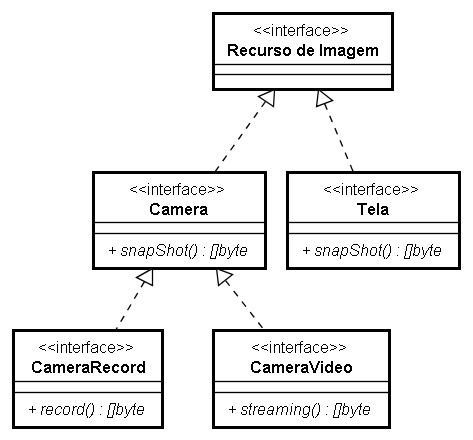
\includegraphics[scale=0.8]{imagens/diagramaRecursosProposta}
	\caption{Exemplos de caso particular da proposta de classificação de recursos.}
	\label{fig:diagramaRecursosProposta}
\end{figure}

\begin{comment}
Suponha que um usuário, por meio de uma aplicação de seu celular, deseja utilizar os serviços providos de um recurso de imagem. Considere ainda, que existam três instâncias disponíveis deste recurso no \emph{smart space}. Para garantir a equivalência dos recursos devemos garantir que eles possuam os mesmos serviços, e para isso, devemos garantir que os serviços possuam a mesma interface, ou seja, os mesmos tipos e número de parâmetros. Suponha que para o usuário que deseja o recurso simples de imagem seja indiferente a quantidade de \emph{megapixels} da imagem. Para o usuário basta apenas o provimento do serviço que retorne algum dado ou altere o estado de alguma aplicação. Dessa forma, devemos garantir que qualquer uma das três instâncias possam prover esse serviço. Uma câmera com \emph{flash}, por exemplo, para este cenário, seria equivalente a um recurso de câmera sem \emph{flash}.
\end{comment}

\section{Equivalência de Recursos}
\label{sec:equivalenciaRecursos}

Entende-se por equivalência tudo aquilo que tem o mesmo valor.

\begin{quote}
	Lucas estava brincando com seu carrinho, quando uma das rodinhas se quebrou. Entristecido, ele procurou por seu pai, que, ao ver a aflição de seu filho, resolveu ajudar. Recolheu uma garrafa PET que estava por perto, desenroscou sua tampinha e a colocou no lugar deixado pela rodinha estragada. Tamanha foi a felicidade de Lucas ao poder voltar a brincar com o seu carrinho.
\end{quote}

A história acima, apesar de simples, contém informações que podem ser úteis. Observe que os objetos envolvidos, ou seja, a rodinha e a tampinha, diferem na maioria das suas características: material, valor, peso, cor, etc. Entretanto, apesar de tudo, pelo menos uma das características é igual: ambas possuem formatos cilíndricos. Foi essa única semelhança que permitiu o conserto do carrinho e garantiu a felicidade de Lucas! Ou seja, no contexto apresentado, a rodinha e a tampinha puderam ser trocadas sem perda de valor.

É exatamente esse o sentido ao se afirmar que dois recursos são equivalentes. Um não precisa ser igual ao outro, mas apenas possuir uma característica que, em determinado momento, possibilite a intercambialidade. Seria possível, por exemplo, utilizar um \emph{joystick} como um dispositivo apontador e, a qualquer momento, substitui-lo por um \emph{laser pointer} de forma que os serviços necessários continuassem sendo providos. Repare que tais dispositivos, assim como a rodinha e a tampinha, são bastante diferentes em diversas de suas características, mas ainda assim são capazes de fornecer serviços iguais, como mover uma seta pela tela.

\subsection{Cálculo de Equivalência}

Para que um recurso R1 seja equivalente a um recurso R2, os serviços de R2 deverão estar presentes no conjunto de serviços de R1, mas R1 poderá ter outros serviços que não estão presentes em R2. Seja S(X), o conjunto de serviços do recurso X, então teríamos que $S(R1) \cap S(R2) = S(R2)$. 

\begin{figure}[ht]
	\center
	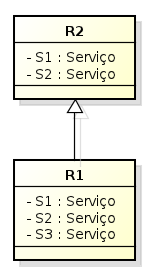
\includegraphics[scale=0.6]{imagens/equivalenciaDeRecursos}
	\caption{Exemplo de recursos equivalentes.}
	\label{fig:equivalenciaDeRecursos}
\end{figure}

Suponha uma situação em que $A \implies B$, $B \implies C$ e $C \implies A$, logo teríamos que $A \implies C$, o que seria uma relação circular, o que não faz sentido, pois concluiríamos que todos os recursos são iguais e não equivalentes. Devemos, portanto, garantir que não ocorra essa equivalência circular. Caso algum dispositivo queira registrar um novo \emph{driver} que cause essa inconsistência, devemos impedir que essa inconsistência possa ocorrer, ou então alertar o novo driver da ocorrência deste problema e não realizar seu registro. 

\subsection{Consistência de Interface}

	A figura~\ref{fig:consistenciaInterface} mostra que o recurso R1 é equivalente ao recurso R3, mas embora possua um serviço de mesmo nome que o recurso R2,  seus parâmetros são diferentes, logo, não pode ser um mesmo serviço e os recursos não serão equivalentes..
	
	Para garantir que os recursos são equivalentes, devemos realizar três validações nas interfaces de cada serviço dos recursos:
	\begin{enumerate}
		\item Recurso:
			
			Os serviços devem pertencer ao mesmo recurso cujas classes padrões foram definidas anteriormente.
		
		\item Identificador do Serviço:

			Os serviços devem possuir os mesmos identificadores.

		\item Parâmetros:

			Os serviços devem possuir os mesmos parâmetros.
	\end{enumerate}

	Parte-se do princípio que não existirá interesse em camuflar um serviço malicioso ao expor uma interface compatível com a equivalência.

\begin{figure}[ht]
	\center
	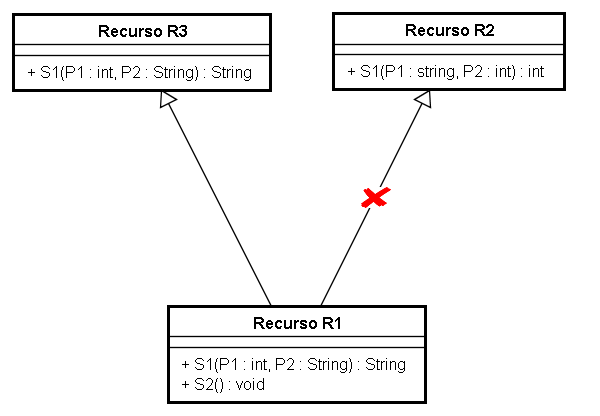
\includegraphics[scale=0.8]{imagens/consistenciaInterface}
	\caption{Exemplo de inconsistência de interface.}
	\label{fig:consistenciaInterface}
\end{figure}

\begin{comment}
----------------------------------------- REVER ----------------------------------------- \\
Desta forma, faz-se necessária uma maneira de classificar tais recursos imersos nos mais variados dispositivos presentes no \emph{smart space} e regidos pelo \emph{middleware}. Essa classificação facilitará o desenvolvimento de novos \emph{drivers} para futuras aplicações, pois tornará possivel a definição de interfaces pré-estabelecidas que representem classes de recursos. Outra vantagem decorrente é a possibilidade de seleção de recursos equivalentes, caso o provedor originalmente selecionado esteja indisponível. \\
----------------------------------------- REVER -----------------------------------------

COLOQUEI NO COMEÇO DA PROPOSTA
\end{comment}

\section{Impacto}
\label{sec:impactoUOS}

A proposta anteriomente definida requer algumas mudanças no \emph{uOS}. Esta seção mostrará um pouco mais sobre como o \emph{uP} foi definido a partir dos conceitos da DSOA e, por fim, mostrará os impactos do uso da classificação para a determinação da equivalência de recursos.

O \emph{uP (Ubiquitous Protocols)} foi construído baseado na arquitetura DSOA. É um conjunto de protocolos criado com objetivo de estabelecer um meio de interação entre os serviços dentro desta arquitetura. Tais protocolos definem o canal de comunicação e a forma de interação entre as entidades do ambiente. As mensagens são transmitidas no formato JSON (\emph{JavaScript Object Notation})~\cite{json}.

\begin{comment}
, que utiliza a codificação UTF-8~\cite{utf8}, que foi escolhido por ser um formato estruturado, leve e independente de plataforma. O JSON foi utilizado ante o XML, pois possui menor tamanho de mensagens e esse fator pode ser decisivo em um ambiente com diversos dipositivos com capacidades computacionais diferentes e possivelmente reduzidas. Dessa forma a limitação dos dispositivos é minimizada e exclui a necessidade de uma rede para tratamento dessas mensagens.
\end{comment}

Cada um dos conceitos apresentados na DSOA possui uma representação no \emph{uP} com seus respectivos atributos:

\begin{itemize}
	\item Dispositivo(\emph{UpDevice}):
	
		Por meio dos seguintes atributos, é possível identificar unicamente o dispositivo no ambiente, e quais são as interfaces rede que o dispositivo possui para realizar alguma comunicação:

	\item \emph{Driver}(\emph{UpDriver}): 

		Representa o conceito do Recurso definido na DSOA. Como um dispositivo pode ter várias instâncias de um recurso, cada instância é identificada unicamente dentro do dispositivo que contém este recurso.

	\item Serviço(\emph{UpService}): 

		Representa o conceito de mesmo nome definido na DSOA.
\end{itemize}

Além disso, com o objetivo de disponibilizar as características de visibilidade, interação e efeito, foram criados mecanismos de acesso aos recursos. O \emph{uP} é dividido em protocolos básicos, que são utilizados para invocar serviços e protocolos complementares que completam suas funcionalidades.

\begin{itemize}
	\item Protocolos Básicos: 

		São divididos em SCP (\emph{Service Call Protocol}) e EVP(\emph{Event Protocol}). O primeiro possui arquitetura provedor-consumidor, ou seja, o consumidor requisita um serviço e o provedor retorna esse serviço para ele de forma síncrona. No último, o consumidor se registra em um evento no provedor, que response informando que o registro foi realizado com sucesso, e na ocorrência do evento, o consumidor é notificado pelo provedor, demonstrando uma forma assíncrona de comunicação.
	\item Protocolos Complementares:

		Além da interação entre os serviços provida pelos protocolos básicos, o \emph{uP} tem mecanismos que permitem que as aplicações obtenham informações sobre quais são os serviços disponíveis no ambiente e informações a respeito deles. Os protocolos são divididos em um grupo de protocolos com informações sobre o dispositivo e um grupo de protocolos com informações sobre o ambiente. 
\end{itemize}

O conceito do Recurso introduzido anteriormente na subseção~\ref{subsec:introUos} do capítulo~\ref{cap:classificacao} será afetado devido a proposta de classificação de recursos. Um dispositivo presente no \emph{smart space}, segundo a DSOA, procura seus serviços no ambiente por meio do identificador do recurso que provê esses serviços. Com a introdução do conceito de Equivalência de Recursos, o dispositivo irá procurar por uma classe desse recurso. O identificador, em vez de representar um nome do recurso, irá, portanto, identificar que tipo de recurso ele representa, ou seja, recurso de: imagem, áudio, apontador e etc. Na visão da DSOA, a interface do recurso foi acrescida da lista de recursos equivalentes. Dessa forma, o recurso fica responsável por informar os recursos aos quais ele é diretamente equivalente. Por exemplo, se $R1 \implies R2$, $R1 \implies R3$ e $R3 \implies R4$, então o recurso $R1$ irá informar que ele é equivalente a $R2$ e $R3$ apenas.

Como \emph{uP} foi criado a partir dos conceitos da DSOA, o impacto sofrido na DSOA foi diretamente refletido sobre ele. Para que a equivalência de serviços possa ser garantida, os recursos do dispositivo, cada um representado por um \emph{UpDriver}, deverá informar os recursos aos quais este é equivalente. Além disso, o identificador do recurso representará a classe deste. Dessa forma, a interface do recurso foi acrescida de um campo para informar estes \emph{drivers}. O \emph{UpDriver} ficará, portanto, com os seguintes campos:

\begin{itemize}
	\item \emph{``name''}:
		
		Representa a classe do recurso.

	\item \emph{``equivalentDrivers''}:
	
		Classes a que este recurso é equivalente.
	\item \emph{``services''}:

		Lista dos serviços síncronos do recurso.

	\item \emph{``events''}:

		Lista dos serviços assíncronos do recurso;
\end{itemize}

O campo \emph{``equivalentDrivers''} irá carregar a informação sobre a equivalência de um recurso. Entretanto, em um ambiente dinâmico, existe a possibilidade do \emph{uOS} não conhecer um destes recursos equivalentes. O dispositivo, então, ficará responsável por prover um serviço que informe ao \emph{uOS} a interface deste(s) recurso(s) desconhecido(s) e sua(s) equivalência(s) até a raiz conhecida pelo \emph{uOS}, para que o \emph{middleware} possa encontrar e registrar este novo driver na árvore de recursos. Para isso, deverá ser criado mais um serviço no protocolo \emph{Device Driver}, um dos protocolos complementares do \emph{uP}, que ficará com os seguintes serviços:

\begin{itemize}
	\item \emph{ListDrivers}: 

		Provê uma lista de instâncias dos drivers disponíveis do dispositivo. Possui dois parâmetros opcionais:
		\begin{itemize}
			\item \emph{``serviceName''}: 

				Nome do serviço;
			\item \emph{``driverName''}: 

				Identificador do recurso.
		\end{itemize}
	\item \emph{Handshake}: 

		Neste protocolo, dois dispositivos trocam informações entre-si. O dispositivo que invoca esse serviço passa como parâmetro um objeto do tipo \emph{device} e recebe como retorno informações sobre o dispositivo que recebeu a chamada;
	\item \emph{Goodbye}: 

		Responsável por retirar o dispositivo da lista de dispositivos presentes no ambiente;
	\item \emph{Authenticate}: 

		Estabelece um contexto de segurança entre dois dispositivos por meio de um prévio compartilhamento de chaves.

	\item \emph{TellEquivalentDrivers}:

		Responsável por informar a interface do(s) recurso(s) desconhecido(s) equivalente(s). Será composto pelos seguintes campos:

		\begin{itemize}
			\item \emph{``driversName''}:

			Lista com o(s) nome(s) do(s) recurso(s).

			\item \emph{``interfaces''}:

			Lista com a(s) interface(s) do(s) recurso(s).
		\end{itemize}
\end{itemize}


\begin{comment}
Serão afetados, ainda, dois protocolos básicos, o \emph{Service Call} e o \emph{Notify}, e o serviço \emph{ListDrivers} dos protocolos \emph{Device Driver} e \emph{Register Driver}. Todos esses serviços contém o parâmetro \emph{driver} que passará a representar uma classe dentre as classes de recursos e não mais o nome do recurso simplesmente.
\end{comment}

Além dos protocolos, que fazem parte do \emph{middleware}, o núcleo do \emph{uOS} ficará responsável por garantir as regras que definirão se dois recursos são equivalentes e, por conseguinte, pelas validações das interfaces dos serviços. Quando um dispostivo entra no ambiente inteligente controlado pelo \emph{uOS}, o \emph{middleware} tenta trocar informações com o dispositivo por meio do serviço ``\emph{handshake}'' do protocolo \emph{DeviceDriver}. Após o ``\emph{handshake}'', o \emph{uOS} busca informações sobre os recursos que aquele dispositivo carrega por meio do serviço ``\emph{listDrivers}''. Antes da introdução da equivalência de recursos, o registro de novos dispositivos parava neste segundo passo. 

O \emph{uOS} a partir de então irá, além de registrar informações sobre o recurso, irá válidar se esse recurso é de fato equivalente à outros recursos analisando uma hierarquia de equivalência. Os recursos definidos neste trabalho representam diferentes raízes na árvore de equivalência. Uma vez que um novo \emph{driver} é implementado e um dispositivo dotado deste recurso adentra ao ambiente inteligente controlado pelo \emph{uOS}, este novo \emph{driver} passa a integrar um novo ``galho'' na árvore de equivalência, caso a definição de seus serviços esteja de acordo com as regras de equivalência e consistência de interfaces.

Quando um dispositivo deseja obter informações sobere os \emph{drivers} de outro dispositivo, ele se utiliza do serviço ``\emph{listDrivers}'', especificando, por exemplo quais \emph{drivers} aquele dispoisito estava procurando. Com a introdução da equivalência de recursos, todos as instâncias do \emph{driver} procurando e todas as insâncias dos \emph{drivers} equivalente a este, serão retornadas como válidas. Ou seja, mesmo que o \emph{driver} requisitado esteja indisponível, seus equivalentes serão capazes de prover os serviços desejados.



  \postextual
  \bibliographystyle{plain}
  \bibliography{bibliografia}

\end{document}
